\subsection*{Hypothesis 1}

\textbf{H0 (Null Hypothesis):} There is a positive correlation between the length of a review and its helpfulness score.\\
\noindent
The data cleaning and 'review/helpfulness' transformation process ($\text{helpfulness score} = \frac{x}{y} \sqrt{y}$) was executed using the `pymongo` library to leverage the efficiency of MongoDB. 
Specifically, we designed a pipeline to perform the necessary operations. Regarding the 'review/text' transformation, we employed the `nltk` 
library to tokenize the text, remove punctuation, stopwords, and subsequently count the number of words.\\
The correlation coefficient between the two variables is 0.3313 with a p-value < 0.05, indicating a statistically significant correlation.
A graphical representation confirming this correlation can be found in Figure \ref{fig:h1_boxplot}. There is a positive correlation observed until 
approximately 400 words, beyond which the boxplot stabilizes. Consequently, we conducted an analysis of the correlation within specific review length 
groups. As a result (Table \ref{corr_groups}), we observed a positive and statistically significant correlation for reviews with lengths between 0 and 400 words. 
However, for reviews longer than 750 words, the correlation becomes negative and statistically significant. For reviews falling in the intermediate range 
(between 400 and 750 words), the correlation is negligible.
\noindent
\textbf{Conclusion:} Our hypothesis is confirmed, but the correlation is not very strong and varies depending on the length of the review.

\begin{figure}[H]
    \centering
    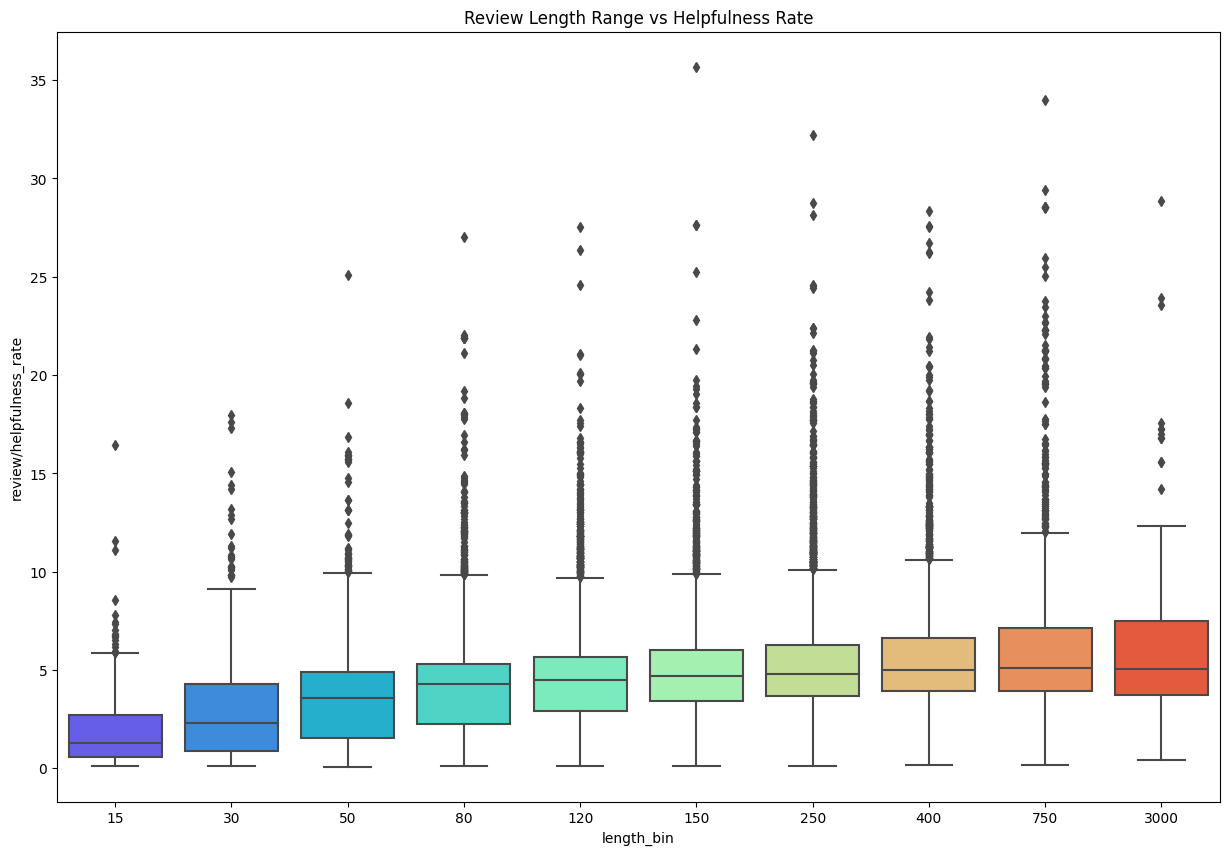
\includegraphics[width=0.49\textwidth]{./figures/h1_boxplot.png}
    \caption{Correlation between review length and helpfulness score for different review length groups}
    \label{fig:h1_boxplot}
\end{figure}

\begin{table}[H]
    \footnotesize
    \centering
    \caption{Correlation Coefficients and P-values for Different Groups}
    \begin{tabular}{|c|c|c|}
    \hline
    Group Number & Correlation Coefficient & P-value \\
    \hline
    400 & 0.2216 & 0.0000 \\
    \hline
    750 & -0.0188 & 0.2585 \\
    \hline
    3000 & -0.1418 & 0.0065 \\
    \hline
    \end{tabular}
    \label{corr_groups}
\end{table}

